\documentclass[conference]{IEEEtran}

\usepackage[T1]{fontenc}
\usepackage{amsmath}
\usepackage{newtxtext,newtxmath}
\usepackage{booktabs}
\usepackage{graphicx}
\usepackage{xcolor}
\usepackage{tikz}
\usepackage{algorithm}
\usepackage{algpseudocode}
\usepackage{microtype}
\usepackage{cite}
\usepackage[hidelinks]{hyperref}

\graphicspath{{figures/}}
\usetikzlibrary{positioning,calc}

\newcommand{\sab}{SA-B\textsuperscript{+}-tree}
\newcommand{\bp}{B\textsuperscript{+}-tree}

\begin{document}

\title{\sab: Stream-Aware Splits and Leaf Hints\\for Append-Heavy B\textsuperscript{+}-Tree Indexes}

\author{\IEEEauthorblockN{Arhaansh Jhingan}
\IEEEauthorblockA{Vellore Institute of Technology, Vellore, India\\
arhaanshjhingan@gmail.com}}

\maketitle

\begin{abstract}
Many indexes receive keys in ascending order: auto-increment identifiers,
timestamps, and composite keys such as (device, time) that are written by many
sources at once. A textbook \bp{} handles this poorly. Every insert descends
from the root, and every split leaves the left page half empty forever.
Production systems patch the single-stream case. PostgreSQL caches the
rightmost leaf, and InnoDB splits at the insertion point when consecutive
inserts are adjacent. Both break down when several streams are interleaved or
when a few records arrive late. We present the \sab, a small, compatible
modification built from three parts: a split rule gated on per-node insert
runs that always cuts just after the run and leaves 10\% headroom on pure
appends; a 64-slot cache of recently written leaves with exact fence keys,
which lets an insert skip the descent; and a hit-rate gate that switches the
cache off when it stops paying. On two million 64-bit keys the \sab{} needs
1.01--1.02 page reads per insert instead of 2.98 and builds an index 43--45\%
smaller. It inserts 2.0--2.5$\times$ faster for sequential, multi-stream and
nearly sorted keys, and stays within 1\% of the textbook tree on random keys.
With 8 or 64 interleaved streams, or 5\% late records, it beats the
combination of the two existing techniques by up to 2.4$\times$ in insert time
and 11--39 percentage points in page fill.
\end{abstract}

\begin{IEEEkeywords}
B+-tree, index maintenance, page splits, fill factor, time-series data
\end{IEEEkeywords}

%======================================================================
\section{Introduction}

The B-tree and its \bp{} variant are the default index of practically every
relational and key--value storage engine~\cite{bayer1972,comer1979,graefe2011}.
Their classic analysis assumes keys arrive in random order. In that case each
insert descends the tree once, and pages settle at about $\ln 2 \approx 69\%$
occupancy~\cite{yao1978}.

Real insert streams are rarely random. Surrogate primary keys come from a
counter. Event tables are keyed by timestamp. Sensor and log tables are often
keyed by a composite such as \texttt{(device\_id, ts)}, so each device appends
to its own region of the key space while thousands of devices write
concurrently. For these \emph{append-heavy} workloads the textbook \bp{} does
two wasteful things:
\begin{enumerate}
\item \textbf{It re-descends for every insert.} The insert lands in the same
  leaf as the previous one, yet it pays $h$ page accesses, where $h$ is the
  tree height.
\item \textbf{It splits in the middle.} When the active leaf overflows, half of
  its keys move to a new right sibling. Later keys are all larger, so they go
  to the right page, and the left page stays 50\% full for good. The index ends
  up twice as large as necessary, and range scans read twice as many pages.
\end{enumerate}

Mature systems ship point fixes. PostgreSQL caches the rightmost leaf and
inserts there directly when the key falls inside it~\cite{pgfastpath}, and it
splits the rightmost page unevenly according to the index
fillfactor~\cite{pgfillfactor}. InnoDB remembers the last insert position on
each page and, when consecutive inserts are adjacent, splits at the insertion
point instead of the middle~\cite{percona2017}. SQLite has a fast ``balance
quick'' path for appending to the rightmost leaf of integer-keyed
tables~\cite{sqlitebtree}. Each fix targets \emph{one} stream at the right edge
of the index. With several interleaved streams the rightmost-leaf cache
almost never hits. The insert-point heuristic is known to under-fill
pages~\cite{mysql67718}, and packing pages completely full backfires as
soon as a few records arrive late.

This paper describes the \sab, a mild but measurable improvement that
generalises these fixes. Our contributions are:
\begin{itemize}
\item a \textbf{run-gated adaptive split} (Section~\ref{sec:split}). It
  activates only after a node has seen a run of adjacent inserts, cuts
  \emph{after} the new key so that keys of a neighbouring stream move out of
  the active page, and keeps a 10\% headroom on pure appends;
\item a \textbf{multi-slot leaf hint cache} with exact fence keys
  (Section~\ref{sec:hints}). It extends the rightmost-leaf fastpath to any 64
  leaves, and a \textbf{hit-rate gate} disables it on workloads without
  locality;
\item a simple \textbf{cost model} that predicts the measured page reads and
  fill to three digits (Section~\ref{sec:model});
\item an \textbf{open-source implementation and evaluation} against the
  textbook \bp{} and against simplified models of the PostgreSQL and InnoDB
  heuristics, with ablations and sweeps over the number of streams and the
  share of late records (Section~\ref{sec:eval}).
\end{itemize}

%======================================================================
\section{Background}
\label{sec:background}

\subsection{Splits and page fill}
A \bp{} leaf holds up to $C$ entries. Inserting into a full leaf creates a
node with $C+1$ entries, which is cut into a left node with $s$ entries and a
right node with $C+1-s$. The first key of the right node becomes the
separator in the parent, and the split can propagate upward. The textbook
choice $s=\lfloor (C+1)/2 \rfloor$ is optimal when the next key is equally
likely to land anywhere. For ascending keys it is the worst choice: the left
node never receives another key, so the steady-state fill is
$\lfloor (C+1)/2\rfloor / C \approx 50\%$.

\subsection{Existing heuristics}
\emph{Rightmost-leaf fastpath (PostgreSQL).} Since 2018, PostgreSQL's nbtree
remembers the block it last inserted into if that block is the rightmost leaf.
The next insert checks that the block is still the rightmost leaf, has free
space, and that the key is greater than the page's first key. If so, it
inserts without descending~\cite{pgfastpath}. A split of the rightmost page
leaves it filled to the fillfactor, 90\% by default for B-tree
indexes~\cite{pgfillfactor}.

\emph{Insert-point split (InnoDB).} InnoDB records the position of the last
insert on each page. If the next insert lands immediately next to it, InnoDB
assumes a sequential pattern and splits at the insertion point, so that the new
record starts the new page~\cite{percona2017}. The heuristic fires on a
single adjacent pair. When the insert point lies in front of keys belonging
to another key range, the next page inherits those keys, and pages can be
drastically under-filled~\cite{mysql67718}.

\emph{Fence keys.} Many \bp{} implementations store, in each node, the
interval of keys it is responsible for: a \emph{high key} as in
Lehman and Yao~\cite{lehman1981}, or both low and high \emph{fence
keys}~\cite{graefe2011}. We use leaf fences to validate hints.

%======================================================================
\section{Design}
\label{sec:design}

The \sab{} is an ordinary \bp{}: same node layout, search, scan and
separator semantics. It differs only in where nodes are split and in how an
insert finds its leaf. Both changes are local to the insert path.

\subsection{Insert-direction tracking}
Every node keeps two small counters, in the spirit of InnoDB's page header
fields: \texttt{last\_pos}, the slot of the most recent insert, and
\texttt{run}, the number of consecutive inserts that landed at
\texttt{last\_pos}$+1$, i.e.\ immediately to the right of the previous one.
Inner nodes track the slots at which separators are inserted in the same way.
An erase resets the counters. After a split, the half that received the new
key inherits the run.

\subsection{Run-gated adaptive split}
\label{sec:split}

\begin{figure}[t]
\centering
\resizebox{\columnwidth}{!}{%
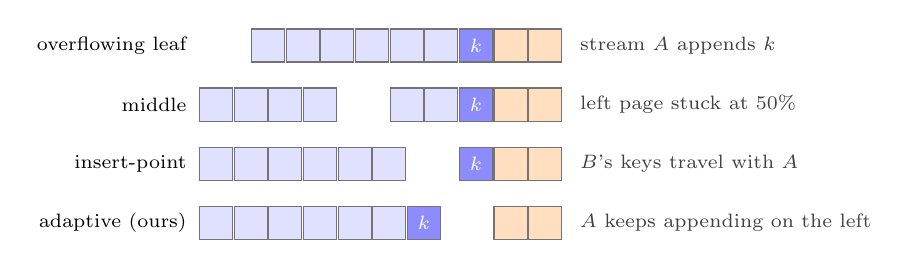
\begin{tikzpicture}[
  cell/.style={draw=black!55, minimum width=4.2mm, minimum height=4.2mm, inner sep=0pt, font=\scriptsize},
  a/.style={cell, fill=blue!12},
  new/.style={cell, fill=blue!45, text=white, font=\scriptsize\bfseries},
  b/.style={cell, fill=orange!25},
  lab/.style={font=\scriptsize, anchor=east},
  note/.style={font=\scriptsize, anchor=west, text=black!75}]
  \def\newtag{new}
  % one row per policy: the left node's cells, a gap, then the right node's
  % cells. All rows end at the same x so the notes line up.
  \newcommand{\splitrow}[5]{% y, label, left cells, right cells, note
    \node[lab] at (-0.25, #1) {#2};
    \foreach \t [count=\i from 0] in {#3}
      \node[\t] at (\i*0.44, #1) {\ifx\t\newtag $k$\fi};
    \foreach \t [count=\i from 0] in {#4}
      \node[\t] at (4.18 - \i*0.44, #1) {\ifx\t\newtag $k$\fi};
    \node[note] at (4.5, #1) {#5};}
  \node[lab] at (-0.25, 0) {overflowing leaf};
  \foreach \t [count=\i from 0] in {a,a,a,a,a,a,new,b,b}
    \node[\t] at (0.66 + \i*0.44, 0) {\ifx\t\newtag $k$\fi};
  \node[note] at (4.5, 0) {stream $A$ appends $k$};
  \splitrow{-0.75}{middle}{a,a,a,a}{b,b,new,a,a}{left page stuck at 50\%}
  \splitrow{-1.5}{insert-point}{a,a,a,a,a,a}{b,b,new}{$B$'s keys travel with $A$}
  \splitrow{-2.25}{adaptive (ours)}{a,a,a,a,a,a,new}{b,b}{$A$ keeps appending on the left}
\end{tikzpicture}}
\caption{Three ways to split a leaf that holds the tail of ascending stream
$A$ (blue) and the head of the neighbouring range $B$ (orange) when $A$'s new
key $k$ overflows it.}
\label{fig:split}
\end{figure}

Let the overflowing node hold $n=C+1$ keys, with the new key at slot $p$.
If the node's run is shorter than a threshold $R$ (we use $R=3$), it splits in
the middle as usual. A random insert lands right after the previous one with
probability about $1/C$, so three in a row virtually never happen by chance.
Otherwise the left node keeps $s$ keys:
\begin{equation}
s=\begin{cases}
p+1 & \text{if } p+1<n \quad\text{(keys follow the run)}\\[2pt]
\lfloor f\,C \rfloor & \text{if } p+1=n \quad\text{(pure append)}
\end{cases}
\label{eq:split}
\end{equation}
The value is clamped so both halves are non-empty; an inner node needs one key
on each side of the key it moves up. Fig.~\ref{fig:split} contrasts the rule
with the alternatives.

\emph{Cutting after the new key} matters when the run sits in front of
someone else's keys, which is the normal state of a composite-key index with
many streams. The keys after $k$ belong to the next range and will never
receive another insert from this stream. Moving them out, rather than moving
$k$ out with them as the insert-point heuristic does, leaves the stream
appending to the end of a page that contains only its own keys. The next
overflow of that page is a pure append.

\emph{The fill limit $f$} applies only to pure appends. With $f=1$ the left
page is packed completely, but a single late record that belongs in it then
forces a middle split, leaving two half-empty pages that never fill up again.
We use $f=0.9$, the same headroom PostgreSQL's default B-tree fillfactor
leaves~\cite{pgfillfactor}. Section~\ref{sec:eval} shows that 1\% late
records are enough to make $f=1$ lose.

The same rule is applied to inner nodes, using the slot at which a separator
is inserted. For a single stream this packs the inner levels as well.

\subsection{Leaf hint cache}
\label{sec:hints}
Every leaf stores fence keys $[\mathit{low},\mathit{high})$, set when the leaf
is created by a split and never changed afterwards: the \sab{} never merges
nodes. Fences of different leaves are disjoint and cover the key space. A
small cache of $K$ slots ($K=64$ by default) remembers recently written leaves
together with their fences. Each slot is stored as a page id, $\mathit{low}$,
and $\mathit{span}=\mathit{high}-1-\mathit{low}$ in a structure-of-arrays
layout, so that testing a slot is a single unsigned comparison
$\mathit{key}-\mathit{low}\le\mathit{span}$.

\begin{algorithm}[t]
\caption{Insert with leaf hints (single-threaded)}
\label{alg:insert}
\begin{algorithmic}[1]
\Procedure{Insert}{$k, v$}
  \If{cache enabled \textbf{or} sampled insert}
    \State $i \gets$ last-used slot if it contains $k$, else scan slots
    \If{$i \neq \bot$ \textbf{and} leaf $L_i$ is not full}
      \State insert $(k,v)$ into $L_i$ \Comment{1 page access}
      \State \Return
    \EndIf
  \EndIf
  \State descend from the root to leaf $L$, recording the path
  \State insert $(k,v)$ into $L$; split by Eq.~\eqref{eq:split} if it overflows
  \State propagate separators up the recorded path
  \State cache the leaf now holding $k$ in slot $i$ (or the LRU slot)
\EndProcedure
\end{algorithmic}
\end{algorithm}

Algorithm~\ref{alg:insert} shows the insert path. A hit costs one page access
instead of $h$. If the cached leaf is full, the insert must split it, which
requires the parent path, so it falls back to a normal descent. That leaf
then shares its slot with whichever half now holds the key: the stream's
next leaf replaces the one it just filled, so one stream occupies one slot.
Whenever a leaf splits, any slot caching it gets the new, smaller
$\mathit{high}$. Cached fences are therefore always exact, and a hit can never
put a key in the wrong leaf. Our invariant checker verifies this after every
test batch.

The PostgreSQL fastpath is the special case $K=1$ restricted to the rightmost
leaf. With $K$ slots, $K$ concurrent streams each keep their active leaf
cached.

\subsection{Hit-rate gating}
Probing costs something. With random keys almost every probe misses, and with
more streams than slots the LRU policy thrashes. Every 64 probes the cache
compares its hit count with half the window. Below that it switches to
\emph{sampling}: only every 64th insert probes and refreshes it. One window of
sampled hits switches it back on. Random workloads therefore probe on about
2.4\% of inserts in our runs, and a workload that turns sequential regains the
cache after a few thousand inserts.

\subsection{Cost model}
\label{sec:model}
Consider one append stream with hints enabled, $f<1$ and tree height $h$.
After an append split, the new right leaf holds $C+1-\lfloor fC\rfloor$
entries and absorbs $\lfloor fC\rfloor$ further inserts before it overflows.
All of them are hits except the last, which reads the full leaf and then
descends. Hence
\begin{equation}
\text{reads per insert} = 1+\frac{h}{\lfloor fC\rfloor}, \qquad
\text{leaf fill} = \frac{\lfloor fC\rfloor}{C}.
\end{equation}
For $C=256$, $f=0.9$, $h=3$ this predicts $1.0130$ reads and $89.84\%$ fill.
We measure $1.0129$ (the tree is shallower early in the load) and $89.84\%$.
For $f=1$ it predicts $1.0117$ and $100\%$; we measure $1.0116$ and $99.99\%$.
The textbook tree pays $h$ reads and reaches 50\% fill.

%======================================================================
\section{Implementation}
\label{sec:impl}
The \sab{} is a header-only C++17 library of about 700 lines. Nodes are
fixed-capacity pages (capacity reserved at allocation, so filling a page
never reallocates) held in a page table indexed by page id. Every node visited
by an operation counts as one logical page read, the standard cost model for
disk-resident indexes. Created or modified nodes count as page writes. Leaves
are chained for range scans. Erase removes the key from its leaf without
rebalancing, as PostgreSQL does until VACUUM, which keeps fences immutable.

The split policy (\textsc{Middle}, \textsc{InsertPoint}, \textsc{Adaptive})
and the hint policy (\textsc{None}, \textsc{Rightmost}, \textsc{Multi}) are
independent options, so the same code base provides the textbook baseline,
models of the PostgreSQL and InnoDB heuristics, their combination, and every
ablation. \textsc{Rightmost} caches only the rightmost leaf, as PostgreSQL
does. \textsc{InsertPoint} starts the new page with the new key whenever the
previous insert was adjacent (run $\ge 1$). This is a simplified model of
InnoDB's heuristic: InnoDB's actual split code differs in details, so this
variant shows how the heuristic behaves, not how InnoDB itself performs.

Correctness is checked by differential tests that drive ten configurations,
with node capacities from 3 to 256, through the same streams of inserts,
overwrites, erases, lookups and range scans as a \texttt{std::map}. After
each batch the tests verify key order, fence keys, uniform leaf depth, the
leaf chain, and that every cached hint still matches its leaf. The suite also
passes under AddressSanitizer and UBSan.

%======================================================================
\section{Evaluation}
\label{sec:eval}

\subsection{Setup}
All experiments insert $N=2\times10^6$ distinct 64-bit keys into an empty
tree with $C=256$ (about a 4\,KiB page of 8-byte keys and 8-byte values), in
memory, on one thread. The machine is an Intel Core Ultra 9 285H laptop
running Linux 7.2, with GCC 16 at \texttt{-O3} and the benchmark pinned to a
performance core. The five key orders are generated deterministically:
\emph{sequential} ($0,1,2,\dots$); \emph{random} (a uniform permutation);
\emph{streams-$K$} ($K$ ascending sequences in disjoint key ranges,
interleaved uniformly at random, like \texttt{(device, ts)} keys);
and \emph{nearly sorted} (ascending, but 5\% of the records are delayed by
1--1000 positions).

Page reads, writes, splits and fill are exact. Insert time is noisy on a
laptop: background load and clock changes only ever add time. Each
configuration is therefore built once untimed and then 7 times, interleaving
the variants so that slow drift hits all of them alike, and we report the
fastest run. Across complete re-runs of the suite, absolute times moved by
up to about 10\%, while the comparisons within one workload were stable.

We compare the textbook tree (\emph{baseline}), the PostgreSQL-style cache
(\emph{rightmost}), the InnoDB-style split (\emph{insert-point}), their
combination (\emph{existing}), our two components alone (\emph{adaptive split},
\emph{multi-hint}), and the full \sab{} ($R=3$, $f=0.9$, $K=64$).

\begin{table*}[t]
\centering
\caption{Two million inserts, $C=256$. Times are best of 7; all other columns are exact.
\emph{Existing} = rightmost-leaf cache + insert-point split.}
\label{tab:main}
\small
\begin{tabular}{@{}l rrr rrr rrr rrr@{}}
\toprule
 & \multicolumn{3}{c}{insert time (ns)} & \multicolumn{3}{c}{page reads / insert}
 & \multicolumn{3}{c}{leaf fill (\%)} & \multicolumn{3}{c}{index size (MiB)} \\
\cmidrule(lr){2-4}\cmidrule(lr){5-7}\cmidrule(lr){8-10}\cmidrule(l){11-13}
workload & base & exist. & \textbf{SA} & base & exist. & \textbf{SA}
 & base & exist. & \textbf{SA} & base & exist. & \textbf{SA} \\
\midrule
sequential      & 23.6  & 8.6   & \textbf{9.4}   & 2.98 & 1.01 & \textbf{1.01} & 50.0 & 100.0 & \textbf{89.8} & 61.5 & 30.6 & \textbf{34.1} \\
random          & 222.5 & 219.8 & \textbf{223.6} & 2.98 & 2.98 & \textbf{2.97} & 70.2 & 70.0  & \textbf{70.2} & 43.8 & 43.9 & \textbf{43.8} \\
8 streams       & 43.4  & 45.0  & \textbf{18.4}  & 2.98 & 2.97 & \textbf{1.01} & 50.0 & 79.0  & \textbf{89.8} & 61.5 & 38.8 & \textbf{34.2} \\
64 streams      & 59.2  & 63.9  & \textbf{26.8}  & 2.98 & 2.98 & \textbf{1.01} & 50.1 & 74.4  & \textbf{89.1} & 61.2 & 41.3 & \textbf{34.5} \\
nearly sorted   & 26.0  & 14.1  & \textbf{13.1}  & 2.98 & 1.10 & \textbf{1.02} & 52.1 & 52.3  & \textbf{91.5} & 59.1 & 58.8 & \textbf{33.5} \\
\bottomrule
\end{tabular}
\end{table*}

\begin{figure*}[t]
\centering
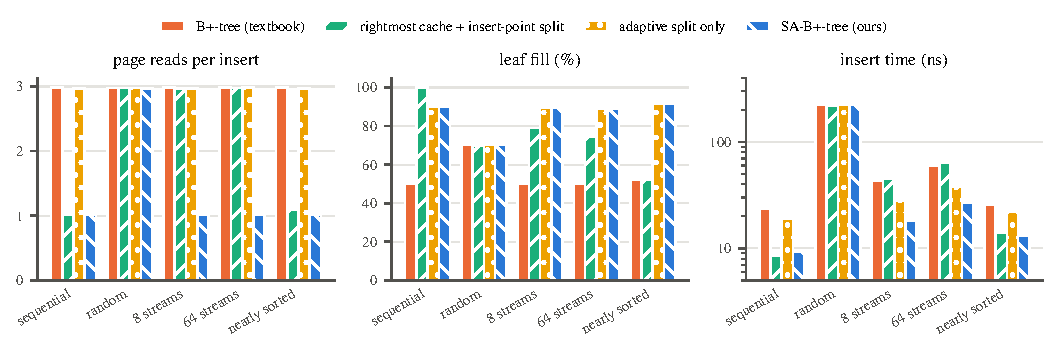
\includegraphics[width=\textwidth]{summary.pdf}
\caption{Page reads per insert, leaf fill and insert time (log scale) for each workload.}
\label{fig:main}
\end{figure*}

\subsection{Overall results}
Table~\ref{tab:main} and Fig.~\ref{fig:main} summarise the main experiment.
On every workload with key locality, the \sab{} needs 1.01--1.02 page reads
per insert instead of 2.98. It builds an index 43--45\% smaller than the
baseline, roughly halves the number of leaf splits (8{,}695 instead of
15{,}623 for sequential keys), and inserts 2.0--2.5$\times$ faster. Smaller
indexes also make range scans cheaper: a scan returning 1{,}000 consecutive
entries reads 7.3--7.4 pages instead of 10.5--10.8. Point lookups cost the
same three page reads in every variant, since all trees have height 3.

On a single clean append stream the existing combination is slightly better
(8.6 vs.\ 9.4\,ns, 30.6 vs.\ 34.1\,MiB). It packs pages to 100\%, which is
exactly what our $f=1$ ablation does too (8.7\,ns, 30.6\,MiB). The 10\%
headroom is a deliberate trade, justified by the next two experiments.
Everywhere else the existing techniques lose most of their benefit. With 8
or 64 interleaved streams the rightmost cache hits almost never, so inserts
still cost 2.97--2.98 reads and the \sab{} is 2.4$\times$ faster. The
insert-point split reaches only 74--79\% fill. With 5\% late records the
cache still works (1.10 reads), but fill collapses to 52\%. On random keys
all variants are within the noise. A dedicated A/B run with 21 interleaved
repetitions measured 224.5\,ns for the \sab{} against 222.4\,ns for the
baseline, a difference of 0.9\%.

\begin{table}[t]
\centering
\caption{Ablation: contribution of each component\\(insert ns\,/\,page reads per insert\,/\,leaf fill \%).}
\label{tab:ablation}
\footnotesize
\setlength{\tabcolsep}{3pt}
\begin{tabular}{@{}lccc@{}}
\toprule
variant & sequential & 64 streams & nearly sorted \\
\midrule
baseline        & 23.6/2.98/50  & 59.2/2.98/50 & 26.0/2.98/52 \\
rightmost       & 11.8/1.02/50  & 60.0/2.98/50 & 14.2/1.10/52 \\
insert-point    & 18.0/2.97/100 & 62.9/2.98/74 & 25.1/2.98/52 \\
adaptive split  & 18.9/2.97/90  & 38.2/2.98/89 & 22.2/2.97/92 \\
multi-hint      & 11.5/1.02/50  & 48.9/1.02/50 & 14.5/1.04/52 \\
\textbf{\sab}   & \textbf{9.4/1.01/90} & \textbf{26.8/1.01/89} & \textbf{13.1/1.02/92} \\
\sab, $f{=}1$   & 8.7/1.01/100  & 26.6/1.01/99 & 14.8/1.03/52 \\
\bottomrule
\end{tabular}
\end{table}

\subsection{Ablation}
Table~\ref{tab:ablation} separates the two components. The adaptive split
alone fixes page fill on every workload and, through fewer splits and better
cache locality, speeds up multi-stream inserts by 1.5$\times$. It does not
reduce page reads. The multi-slot hint cache alone brings reads down to
1.02--1.04 but leaves pages half full. The two are complementary: the
combination is faster than either part on all three workloads.

\begin{figure*}[t]
\centering
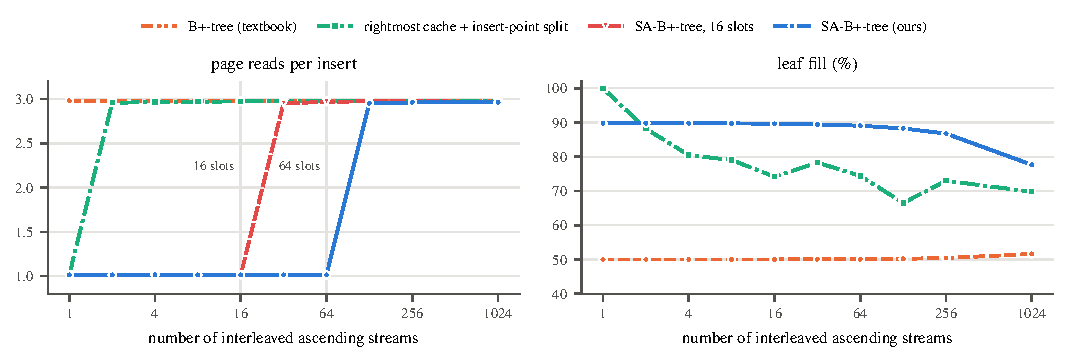
\includegraphics[width=\textwidth]{streams.pdf}
\caption{Sweep over the number of interleaved ascending streams. The \sab{}
with 64 and with 16 hint slots; fill is identical for both and for the
adaptive split alone, so only one curve is drawn on the right.}
\label{fig:streams}
\end{figure*}

\subsection{Number of streams}
Fig.~\ref{fig:streams} varies the number of interleaved streams from 1 to
1{,}024. The hint cache serves 99.6\% of inserts as long as the number of
streams does not exceed its slots: up to 16 streams with $K=16$, up to 64 with
$K=64$. Beyond that the gate switches it off and page reads return to the
baseline. The rightmost-leaf cache already fails at two streams. The adaptive
split keeps leaves 87--90\% full up to 256 streams and 78\% at 1{,}024. The
insert-point heuristic drops to 67--88\% (74\% at 64 streams), the
under-filling described in MySQL bug \#67718. Even past the cache's
capacity (128--1{,}024 streams), the \sab{} remains 1.5$\times$ faster than
the baseline thanks to the split rule alone.

\begin{figure}[t]
\centering
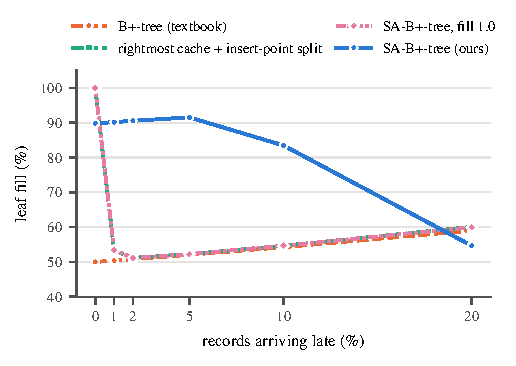
\includegraphics[width=\columnwidth]{late.pdf}
\caption{Leaf fill as a growing share of records arrives up to 1{,}000
positions late. The curves for $f=1$ and for the existing combination
coincide.}
\label{fig:late}
\end{figure}

\subsection{Late records}
Fig.~\ref{fig:late} delays a growing share of records by up to 1{,}000
positions. Any scheme that packs pages to 100\% (the existing combination and
our $f=1$ ablation) falls from 100\% to 53\% fill with only 1\% late records.
Each straggler that lands in a full page splits it in the middle, into two
halves that are never filled again. With $f=0.9$ the \sab{} holds 90--92\%
fill up to 5\% late records and 84\% at 10\%. At 20\% the headroom is no
longer enough: fill drops to 55\%, below the baseline's 59\%. The page-read
saving survives (1.04 reads per insert), but the space saving does not.

%======================================================================
\section{Related Work}
B-trees and their maintenance are surveyed by Comer~\cite{comer1979} and
Graefe~\cite{graefe2011}. Yao's analysis gives the $\ln 2$ fill of random
insertions~\cite{yao1978}. B*-trees~\cite{knuth1998} raise fill by
redistributing keys to siblings before splitting, which helps random inserts
but does not remove the descent cost of appends. Lehman and Yao introduced
per-node high keys for concurrent traversal~\cite{lehman1981}. We reuse the
same idea, as fence keys, to validate cached leaves. Bulk loading builds
packed trees from sorted input, but only when the whole input is available
up front. Write-optimised structures such as the LSM-tree~\cite{oneil1996}
change the storage layout altogether. The \sab{} instead keeps the \bp{}
layout and on-disk format unchanged, so it could replace the insert path of
an existing engine. The closest work is the engineering in PostgreSQL,
InnoDB and SQLite discussed in Section~\ref{sec:background}, which the \sab{}
generalises from one stream at the right edge to many streams anywhere in the
key space.

%======================================================================
\section{Limitations and Future Work}
The evaluation is in memory and single-threaded. In a real engine a skipped
descent also saves latch acquisitions and buffer-pool lookups, so our timings
are probably conservative, but we have not measured that. A concurrent
version would validate a hinted leaf's fences after latching it, the same
check PostgreSQL performs on its cached block. Only ascending runs are
detected; descending runs need a separator chosen just above the left half's
largest key and are left for future work. Nodes are never merged, which keeps
fences immutable outside splits. Supporting merges would require invalidating
the hints of merged pages. At 20\% late records the fixed 10\% headroom stops
working. A natural extension is to stop applying the fill limit to a node once
it observes many out-of-order inserts. Finally, separators of different
streams interleave inside inner nodes, so runs there are short. At 64
streams inner-node fill is 56\% instead of the baseline's 83\%, which has no
practical effect because inner nodes are under 1\% of the pages.

%======================================================================
\section{Conclusion}
Two inexpensive changes to the insert path of a \bp{} recover most of the
waste of append-heavy workloads. A split rule gated on observed insert runs,
which cuts after the run and keeps a little headroom, keeps pages about 90\%
full. A small, self-disabling cache of leaves with exact fences removes the
root-to-leaf descent. Together they cut page reads per insert from about 3 to
1.01, shrink the index by 43--45\% and speed up inserts 2.0--2.5$\times$.
Unlike the single-stream heuristics in production systems, they keep working
with dozens of interleaved streams and with a few percent of late records, and
they cost about 1\% on random keys. The code, benchmarks and raw results are
available at \url{https://github.com/XArhaanshX/database-project}.

\bibliographystyle{IEEEtran}
\bibliography{refs}

\end{document}
